\section{Physics of Proton-Proton Collisions}
\label{sec:Intro_ppCollisions}

Consider a $pp$ collision at LHC. The proton energies are so high that each proton behaves as a complex structure. A proton is a baryon, it consists of three quarks: $uud$. These three quarks are called valence quarks. They interact with each other by exchanging gluons which produce virtual $q\bar{q}$ pairs (Fig.~\ref{fig:ppCollision}). Such virtual quarks are also called sea quarks. \\

Any parton, quark, antiquark or gluon, from one proton can interact with any parton from another proton. Probabilities $f_i(x,Q^2)$ of any particular constituent $i$ to interact are described partially by QCD and partially by experimental measurements and depend on the momentum transfer $Q$ and the momentum fraction of a specific parton $x$. These probabilities are called parton distribution functions (PDFs).\\

\begin{figure}[htb]
  \begin{center}
    {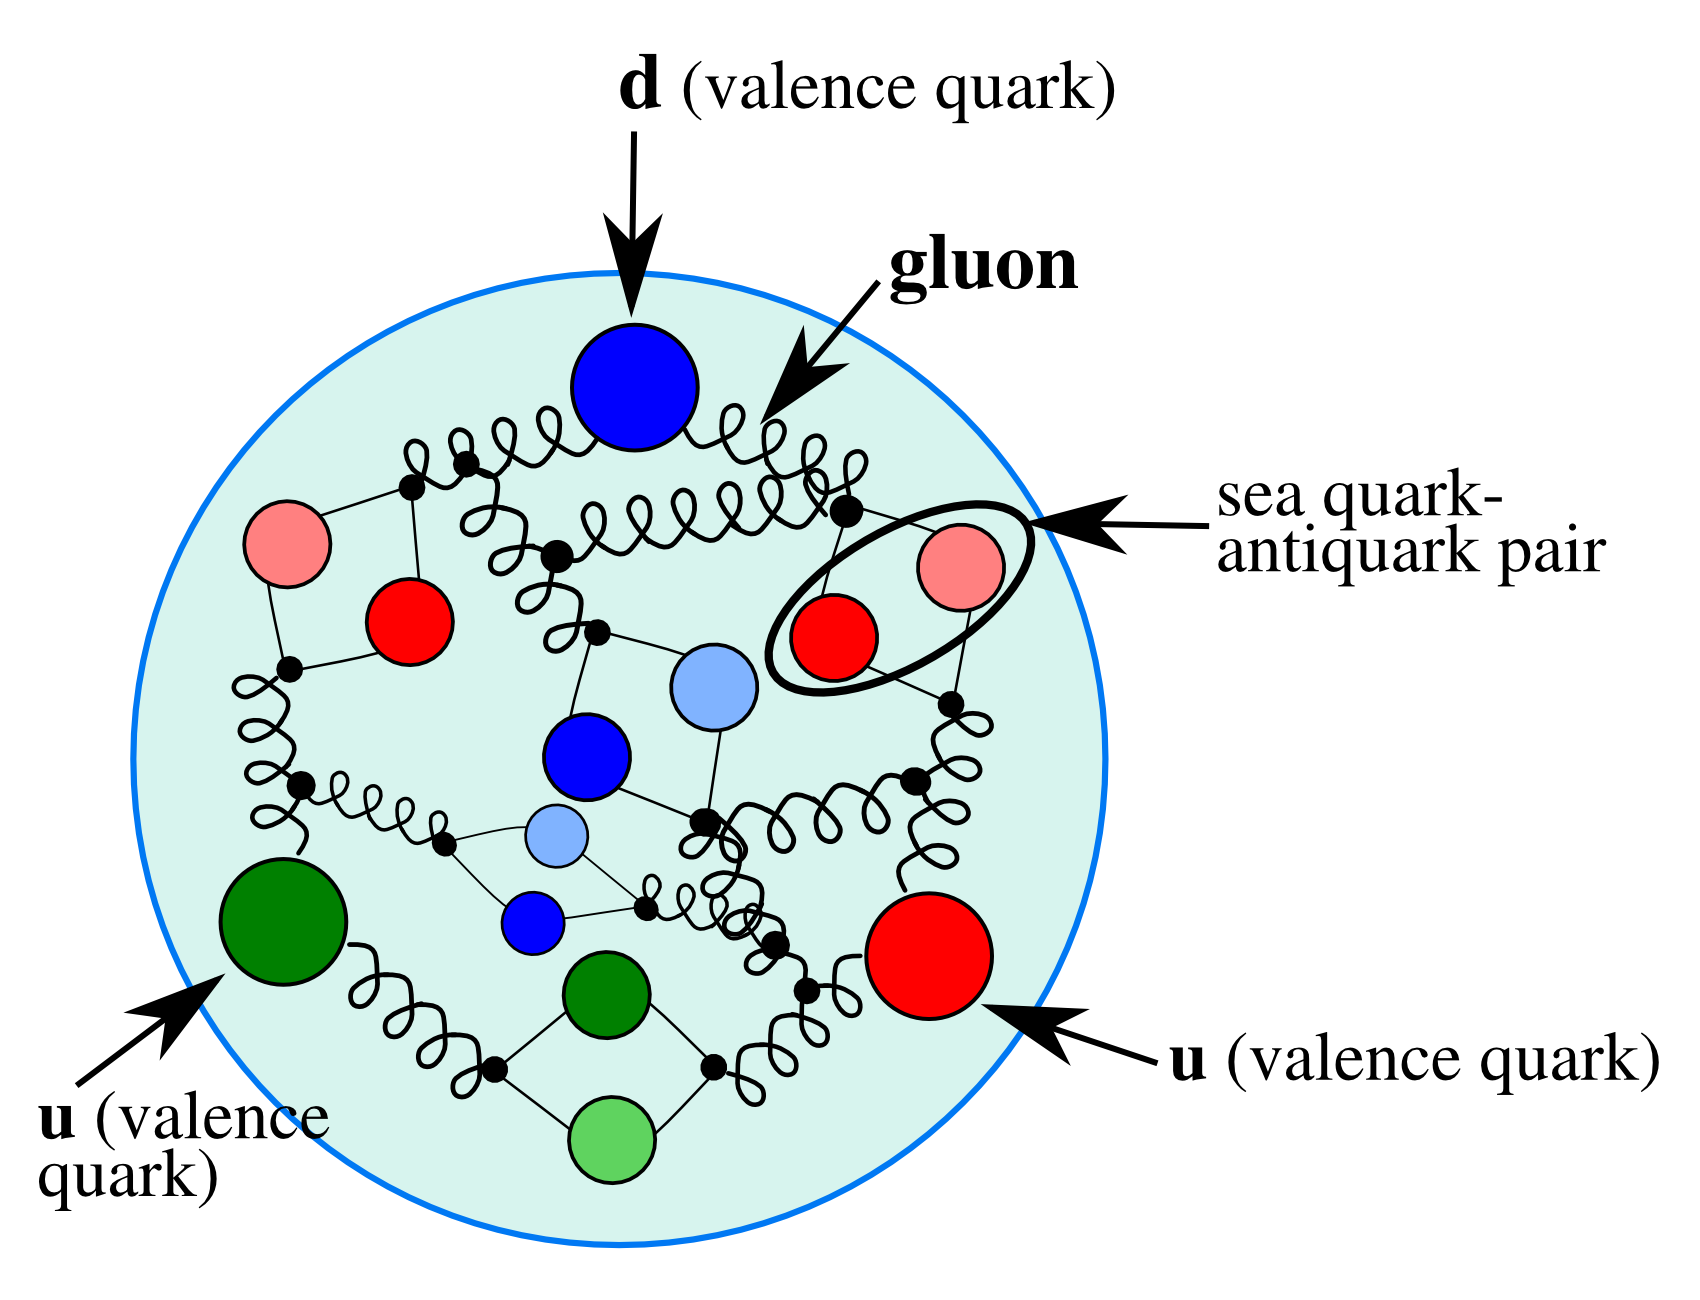
\includegraphics[width=0.45\textwidth]{../figs/Intro/protonStructure.png}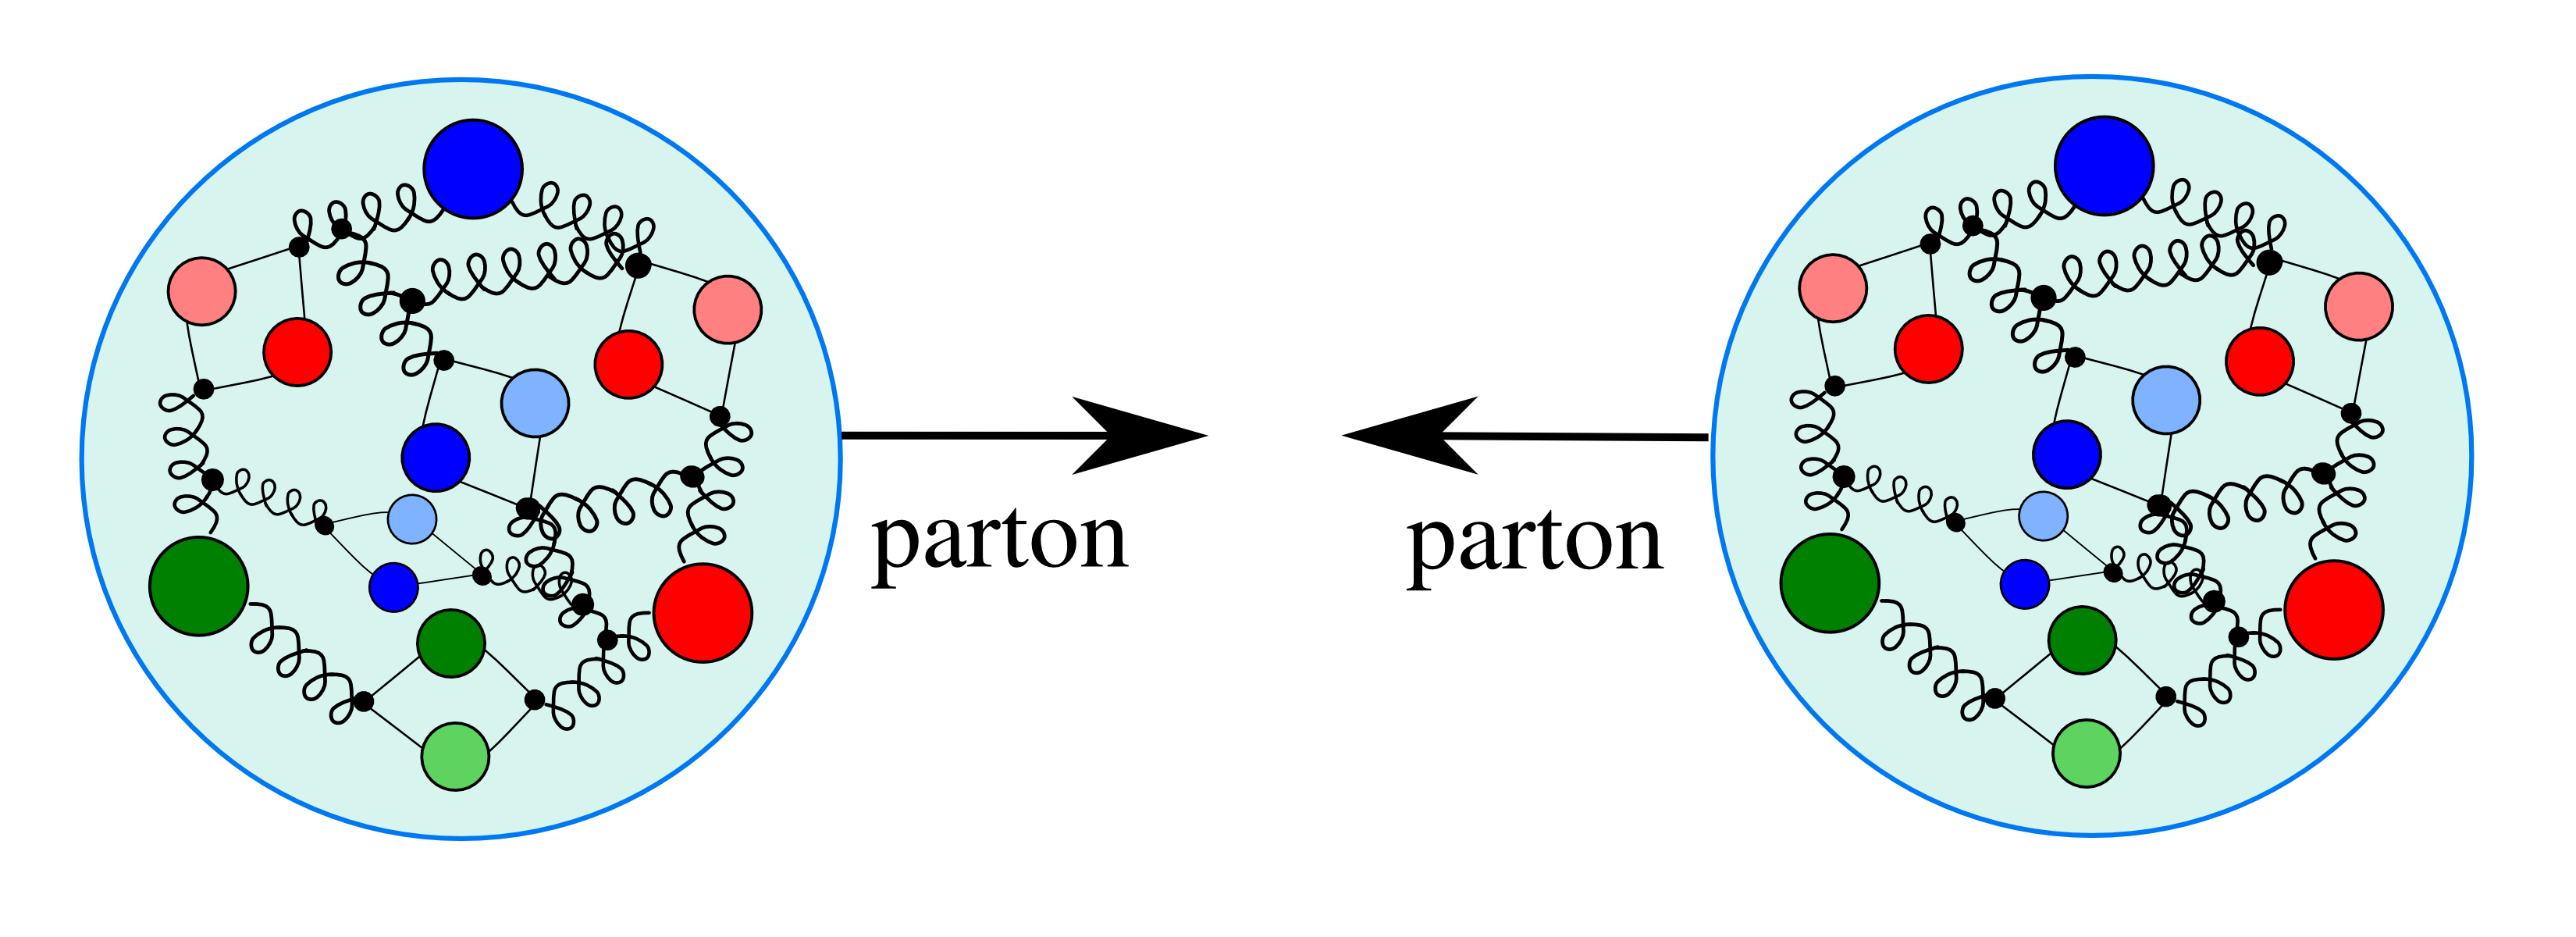
\includegraphics[width=0.45\textwidth]{../figs/Intro/ppCollision.png}}
    \caption{The proton structure (left) and the proton-proton collision (right).}
    \label{fig:ppCollision}
  \end{center}
\end{figure}

\begin{figure}[htb]
  \begin{center}
    {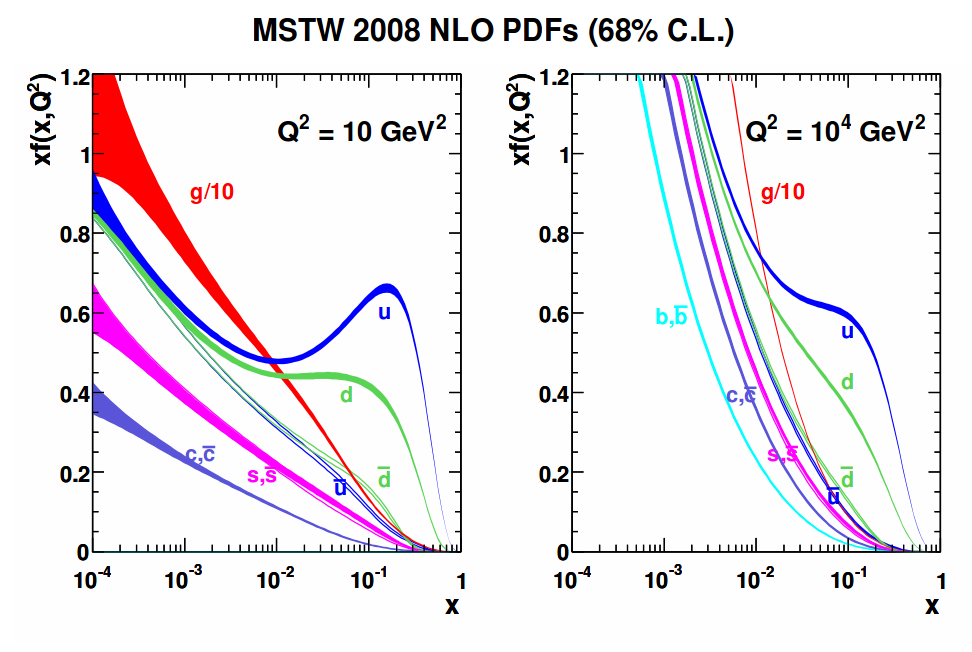
\includegraphics[width=0.85\textwidth]{../figs/Intro/pdfs.png}}
    \caption{Parton distribution functions~\cite{ref_PDG}.}
    \label{fig:pdfs}
  \end{center}
\end{figure}

For large $Q^2$ and $x$ gluon-gluon interactions have the largest probabilities to occur (Fig.~\ref{fig:pdfs}). However, gluons do not couple directly to a $W$ boson, thus, in the $W\gamma$ measurement we are mostly interested in quark-antiquark pairs which would have a total charge corresponding to the charge of a $W$ boson ($\pm 1$). Since we have $u$ and $d$ as valence quarks and we know that the probability to couple to the same generation quark in charged weak interactions is the highest, most of the $W$ bosons are created by $u\bar{d}$ and $d\bar{u}$ pairs however other $q\bar{q'}$ combinations with the total charges of $\pm 1$ are also possible. As we look for events containing $W\gamma$ we also have other events mimicking our process. Such background events can be produced by any pair of partons.\\


% ADD FIGURE WITH PDFs LIKE IN THE PRESENTATION

